\newpage
\subthesischapter{Diseño de la base de datos}
Existen dos tipos prominentes de sistemas de gestión de bases de datos ampliamente reconocidos: los conocido como Lenguaje de Consulta Estructurado (SQL, por sus siglas en inglés) organizan los datos en estructuras tabulares, mientras que los otros, denominado No-SQL, prescinden de las tablas y optan por almacenar datos en forma de objetos. Contrariamente a SQL, el enfoque No-SQL no sigue una estructura rígida, permitiendo mayor flexibilidad en la organización de los datos. No obstante, se ha observado que los sistemas No-SQL tienden a requerir una mayor cantidad de recursos computacionales en comparación con las implementaciones SQL. En el contexto de aplicaciones móviles, se ha preferido el uso de SQL debido a su eficiencia y menor consumo de recursos, lo que contribuye a una experiencia de usuario más fluida y eficaz.

\subsubthesischapter{Modelo lógico}
La descripción que surge de esta fase de diseño sirve como base para especificar la estructura conceptual de la base de datos. 
La siguiente lista describe los principales requisitos para el registro de datos en el sistema:
\begin{itemize}
    \item Los usuarios son reconocidos a través de un identificador único. En el sistema, se almacenan los detalles de identificación del usuario, los cuales se especifican en los requisitos de registro e incluyen el nombre completo, su dirección de correo electrónico y una contraseña asociada.
    \item Cada usuario tiene la capacidad de establecer múltiples rutinas de entrenamiento personalizadas. Estas rutinas están compuestas por un identificador exclusivo, el tipo de ejercicio elegido y los parámetros específicos que han sido configurados por el usuario. 
    \item Luego de terminada una rutina se almacena en el sistema los resultados obtenidos y la fecha de ejecución. 
\end{itemize}   
    
\textbf{Designación de los conjuntos de entidades y de relaciones}\\
Desde la especificación listada anteriormente se comienzan a
identificar los conjuntos de entidades y relaciones, así como sus atributos:
\begin{itemize}
    \item La entidad \underline{usuario}, con los atributos id\_usuario, nombre, correo, contraseña.
    \item La entidad \underline{rutina} con los atributos id\_rutina, modalidad, distancia, tiempo, \textbf{mcv\textsubscript{0}, mcv\textsubscript{1}, mcv\textsubscript{2}, mcv\textsubscript{3}}\footnote{mcv\textsubscript{i}: Valor porcentual definido de MCV en el canal i luego de la etapa de calibración.}.
    \item La relación muchos a muchos de \underline{usuario} a \underline{rutinas} denominado \underline{ejecuta}, es decir un usuario puede ejecutar 
    varias rutinas y la misma rutina puede ser ejecutada por distintos usuarios. Dicha relación cuenta con los atributos velocidad, mcv\_promedio y fecha\_de\_ejecución. 
\end{itemize}
    
El diagrama Entidad-Relación (E-R) que resulta de tales especificaciones para la descripción de los datos del sistema se presenta en la figura~\ref{fig: diagram-er}.
\begin{figure}[ht]
    \centering
    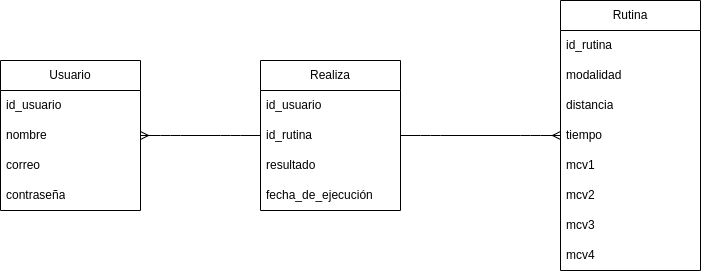
\includegraphics[scale=0.48]{images/diagram-er.png}
    \caption{Diagrama Entidad Relación}
    \label{fig: diagram-er}
\end{figure}

\subsubthesischapter{Modelo físico}
El modelo físico de la base de datos consta de tres tablas principales: \textbf{USER, RUTINE y DO}\footnote{USER, RUTINE y DO hace referencias a las tablas usuario, rutina y ejecuta respectivamente.} en las que se han definido las siguientes restricciones para mantener la integridad de los datos:

\begin{itemize}
    \item En la tabla USER, se ha establecido un campo ID como clave primaria, que se genera automáticamente mediante autoincremento cada vez que se inserta una nueva fila. Los campos FULLNAME, EMAIL y PASSWORD almacenan la información del usuario.

    \item La tabla RUTINE contiene información sobre las rutinas de ejercicios. Se ha definido un campo ID como clave primaria con autoincremento. Los campos MODALITY, TIME, DISTANCE, MCV0, MCV1, MCV2 y MCV3 almacenan los detalles de la rutina.

    \item En la tabla DO, se ha establecido un campo ID como clave primaria con autoincremento. Los campos ID\_MODALITY y ID\_USER actúan como claves foráneas, haciendo referencia a las tablas RUTINE y USER respectivamente. El campo VELOCITY y MCV\_AVERAGE almacena los resultados de velocidad y el promedio de MCV obtenidos al finalizar la rutina, y el campo DATE registra la fecha de la realización de la rutina.
\end{itemize}

El esquema de las tablas de la base de datos, junto con las dependencias de clave primaria y las foráneas, se puede visualizar en la siguiente 
porción de código:

\begin{center}
\begin{minipage}{0.8\textwidth}
\begin{lstlisting}[language=c,caption={Sección de código, constructor de la clase CibiofibDb}, label={code: database-code}]
public CibiofibDb() : base()
{
    IDbCommand dbcmd = getDbCommand();
    dbcmd.CommandText = "CREATE TABLE IF NOT EXISTS USER ( " +
                        "ID  INTEGER PRIMARY KEY AUTOINCREMENT, " +
                        "FULLNAME TEXT, " +
                        "EMAIL TEXT, " +
                        "PASSWORD TEXT )";
    dbcmd.ExecuteNonQuery();

    dbcmd = getDbCommand();
    dbcmd.CommandText = "CREATE TABLE IF NOT EXISTS RUTINE ( " +
                        "ID  INTEGER PRIMARY KEY AUTOINCREMENT, " +
                        "MODALITY INTEGER, " +
                        "TIME REAL, " +
                        "DISTANCE REAL, " +
                        "MCV0 REAL, " +
                        "MCV1 REAL, " +
                        "MCV2 REAL, " +
                        "MCV3 REAL )";

    dbcmd.ExecuteNonQuery();

    dbcmd = getDbCommand();
    dbcmd.CommandText = "CREATE TABLE IF NOT EXISTS DO ( " +
                    "ID  INTEGER PRIMARY KEY AUTOINCREMENT, " +
                    "USER_ID INTEGER, " +
                    "RUTINE_ID INTEGER, " +
                    "VELOCITY REAL, " +
                    "MCV_AVERAGE REAL, " +
                    "DATE TEXT, " +
    "FOREIGN KEY(USER_ID) REFERENCES USER(ID), " +
    "FOREIGN KEY(RUTINE_ID) REFERENCES RUTINE(ID))";

    dbcmd.ExecuteNonQuery();
}
\end{lstlisting}
\end{minipage}
\end{center}